\documentclass{beamer}

\usepackage{amsmath}
\usepackage{mathtools}
\usepackage{amsfonts}
\usepackage{amssymb}
\usepackage{url}
\usepackage{caption}
\usepackage{subcaption}
\usepackage{svg}

\usetheme{default}

\title{Sensor Network for Smart Agriculture}
\author{Jiří Maňák}
\date{\today}

\setbeamertemplate{navigation symbols}{}
\setbeamertemplate{footline}[page number]{}
\addtobeamertemplate{footline}{
    ~~~~\small{\url{manakjiri.cz/thesis}}
}{}

\begin{document}


\begin{frame}
\titlepage
\end{frame}


\begin{frame}{Live Demo}
\begin{figure}
    \centering
    
\includegraphics[width=.5\linewidth]{img/qr.png}
\end{figure}
\begin{center}
    (or visit the link)
\end{center}
\end{frame}


\begin{frame}{Motivation}
\begin{figure}
    \centering
    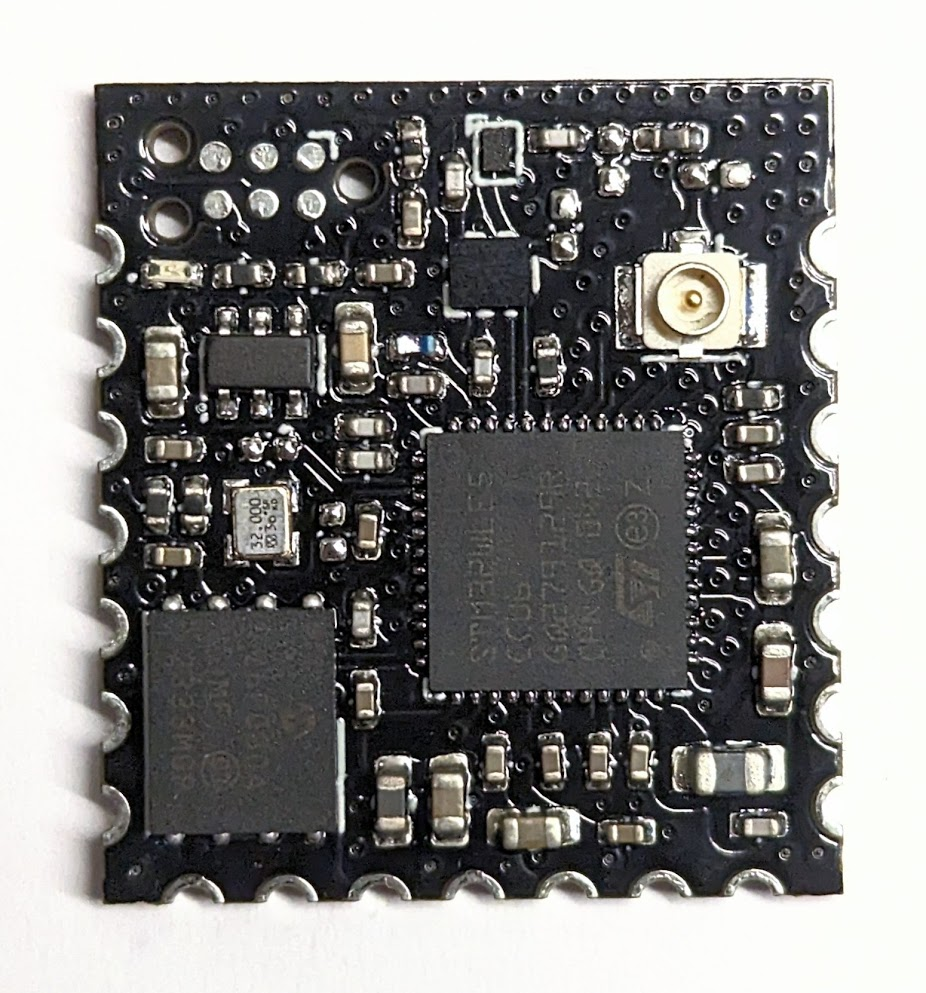
\includegraphics[width=.65\linewidth]{img/module-v0.1.jpg}
\end{figure}
\end{frame}


\begin{frame}{Goals}
\begin{columns}[T]
\begin{column}{.5\textwidth}
    Generic LoRa Module
    \begin{itemize}
        \item Design the PCBA
        \item Implement OTA update
        \item Validate wireless performance
    \end{itemize}
\end{column}
\hfill
\begin{column}{.5\textwidth}
    Soil Moisture Sensor
    \begin{itemize}
        \item Find suitable form--factor
        \item Design measurement circuit
        \item Design power management
    \end{itemize}
\end{column}
\end{columns}
$$\underbrace{\text{\hspace{20em}}}_{}$$
\begin{center}
    Implement and Test the MVP
\end{center}
\end{frame}


\begin{frame}{LoRa Module}
\begin{itemize}
    \item 2.8--3.3 V nominal voltage range,
    \item low power design - support for switchable power rails,
    \item target the EU868,
    \item wide temperature range
    \item minimize the amount of specialized hardware,
    \item support for OTA updates,
    \item integrated RF,
    \item host communication interface,
    \item minimal footprint,
    \item low cost.
\end{itemize}
\begin{flushright}
    Page 15, Section 3.2.3
\end{flushright}
\end{frame}


\begin{frame}{LoRa Module}
\begin{figure}
    \centering
    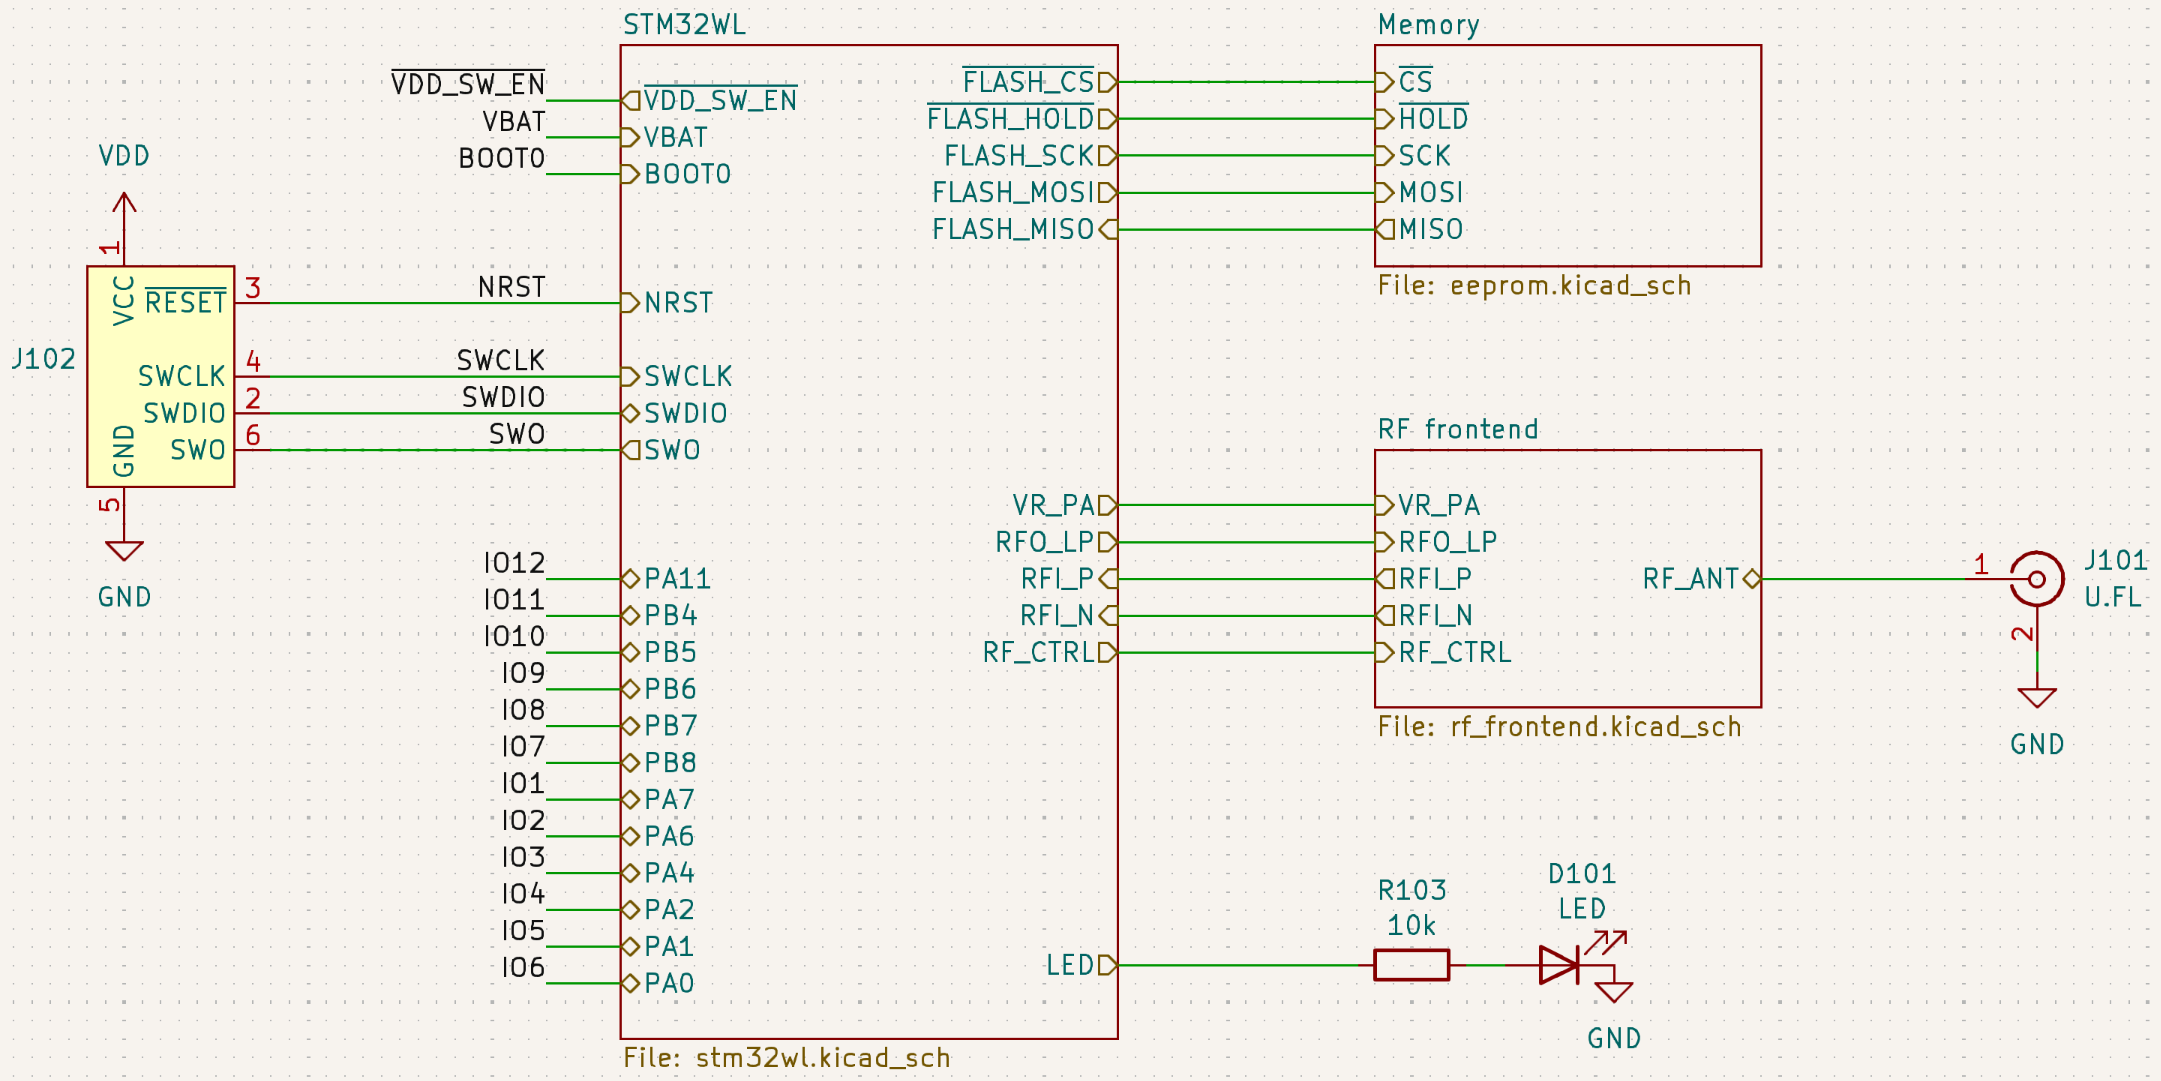
\includegraphics[width=\linewidth]{img/module-schema.png}
\end{figure}
\end{frame}


\begin{frame}{LoRa Module}
\begin{columns}[T]
\begin{column}{.3\textwidth}
    \centering
    \begin{figure}
        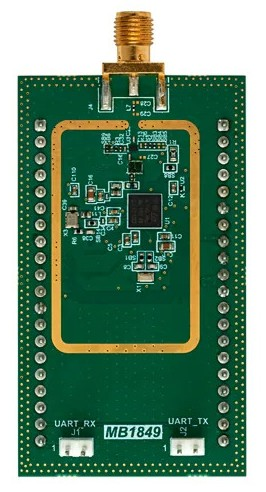
\includegraphics[width=.9\linewidth]{img/STDES-WL5U4ILH.jpg}
    \end{figure}
    STDES-WL5U4ILH
\end{column}
\hfil
\begin{column}{.3\textwidth}
    \centering
    \begin{figure}
        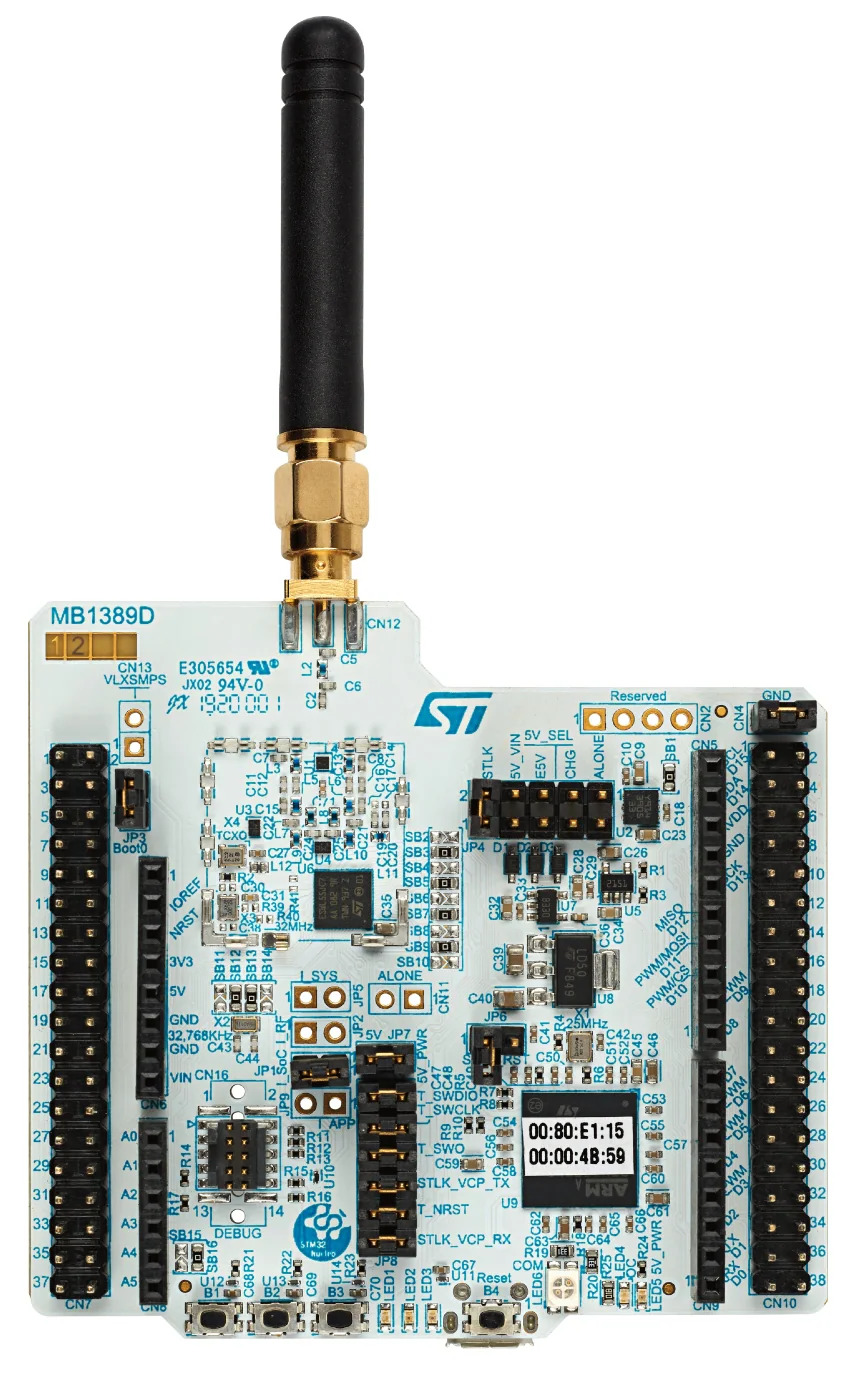
\includegraphics[width=\linewidth]{img/nucleo-wl55jc.jpg}
    \end{figure}
    Nucleo-WL55JC
\end{column}
\end{columns}
\end{frame}


\begin{frame}{LoRa Module}
\begin{figure}
    \centering
    \small
    \includesvg[width=.8\linewidth]{img/module-v0.1.drawio.svg}
\end{figure}
\begin{columns}[T]
\begin{column}{.5\textwidth}
    \begin{itemize}
        \item STM32WLE5CC
        \item 868 MHz, 13 dBm
        \item 20.32 $\times$ 22.48 mm
    \end{itemize}
\end{column}
\hfill
\begin{column}{.5\textwidth}
    \begin{itemize}
        \item 1 MB FLASH
        \item 2.3--3.5 V
        \item 16 IO pins
    \end{itemize}
\end{column}
\end{columns}
\end{frame}


\begin{frame}{Existing solution?}
\begin{columns}
\begin{column}{.4\textwidth}
    \centering
    \begin{figure}
        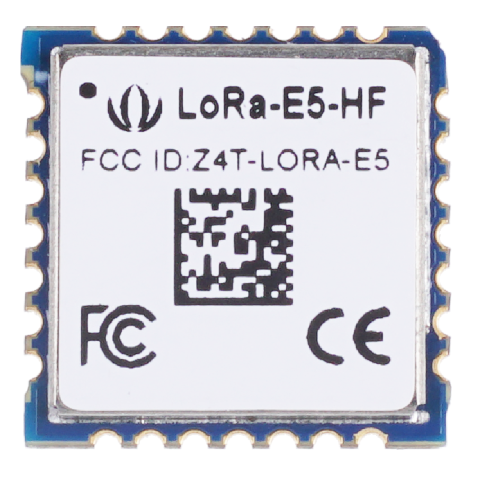
\includegraphics[width=\linewidth]{img/wio-e5.png}
    \end{figure}
    Seeed Studio Wio-E5
\end{column}
\hfil
\begin{column}{.1\textwidth}
    \centering
    \Large
    \vspace{-2em}
    $$>$$
    ?
    $$<$$
\end{column}
\hfil
\begin{column}{.4\textwidth}
    \centering
    \begin{figure}
        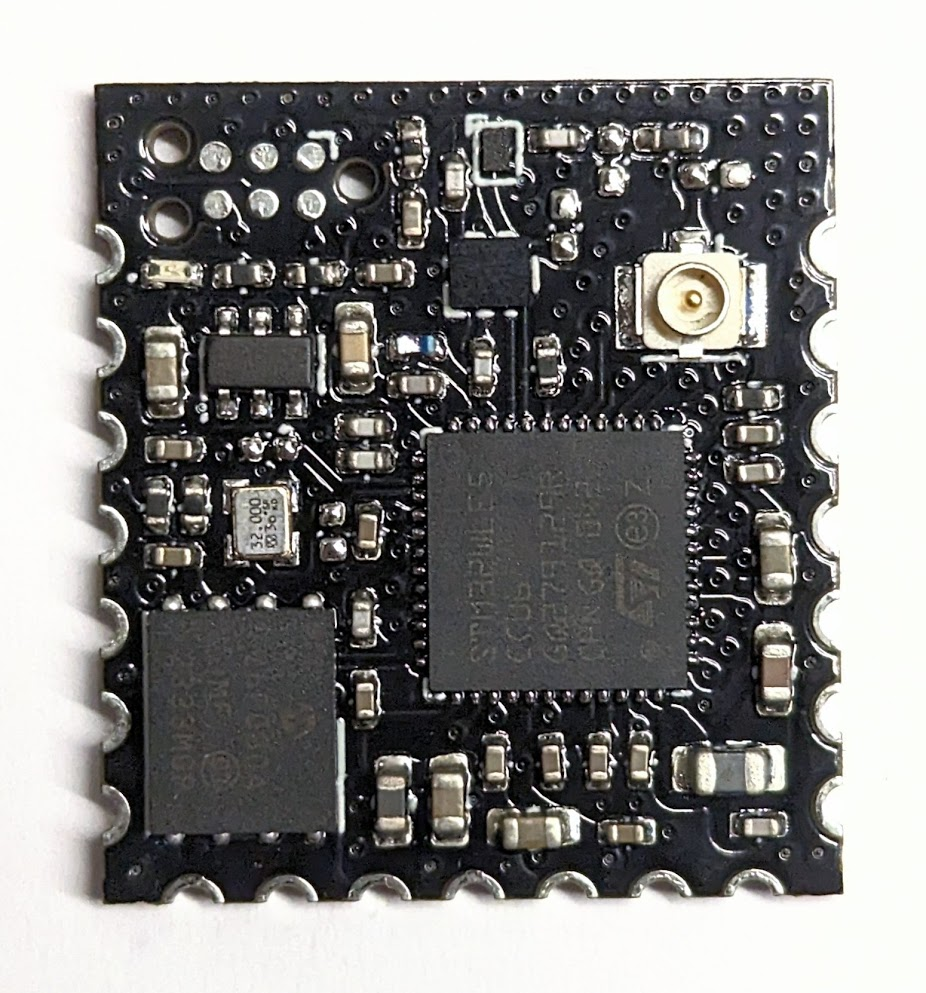
\includegraphics[width=\linewidth]{img/module-v0.1.jpg}
    \end{figure}
    My LoRa Module
\end{column}
\end{columns}
\end{frame}


\begin{frame}{Firmware}
\begin{figure}
    \centering
    \includesvg[width=\linewidth]{img/firmware.drawio.svg}
\end{figure}
\end{frame}


\begin{frame}{Over The Air Update}
\begin{figure}
    \centering
    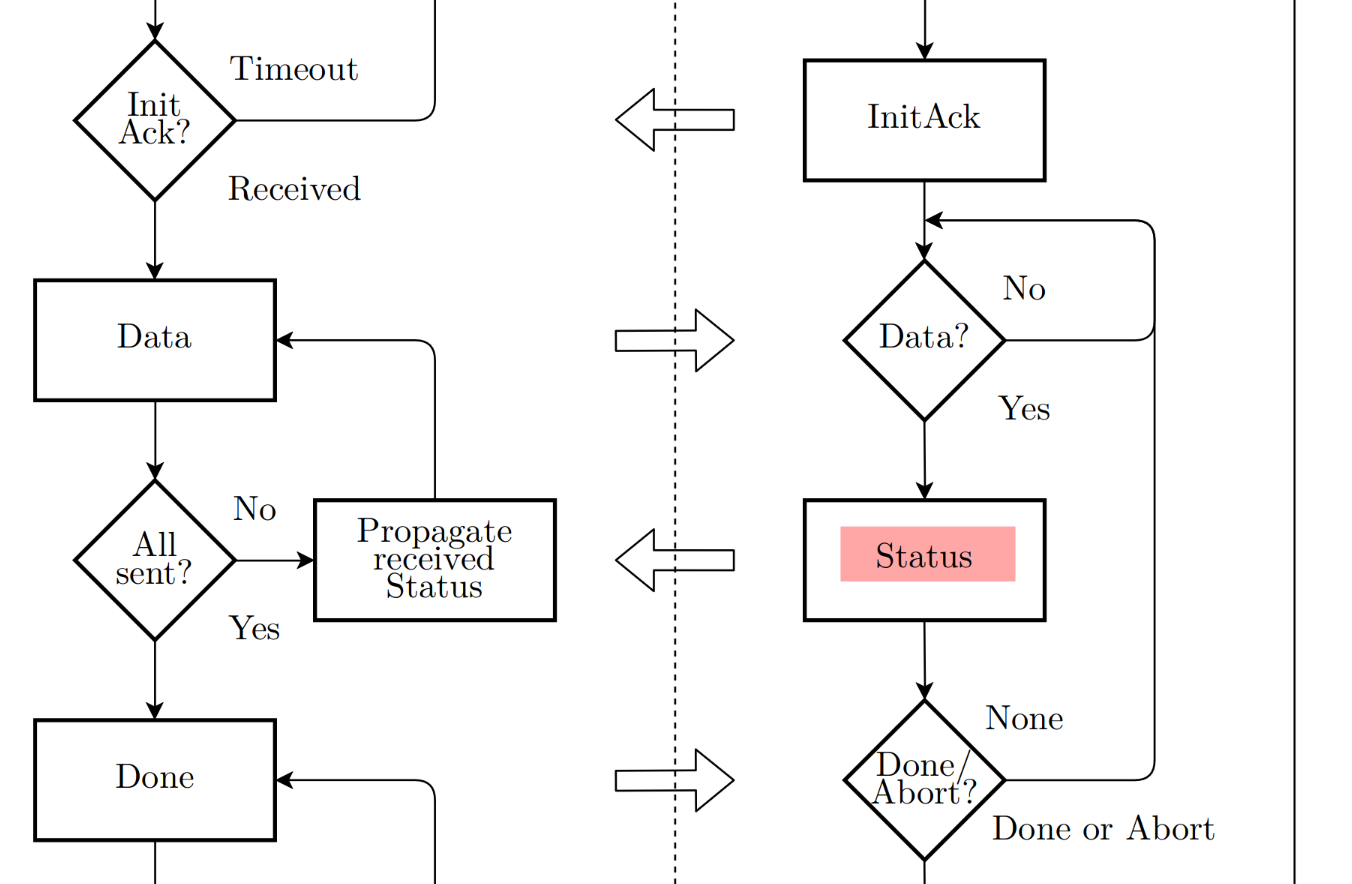
\includegraphics[width=\linewidth]{img/ota.png}
\end{figure}
\begin{flushright}
    Page 36, Figure 4.9
\end{flushright}
\end{frame}


\begin{frame}{Soil Moisture Sensor}
\begin{itemize}
    \item PCB construction
    \item 4 capacitive zones (15 cm total depth)
    \item Solar powered
\end{itemize}
\begin{figure}
    \centering
    \includesvg[width=\linewidth]{../thesis/boards/sensor/soil-sensor-F_Cu.svg}
\end{figure}
$$\underbrace{\text{\hspace{5em}}}_{\text{Sensor electronics}}~\underbrace{\text{\hspace{19em}}}_{\text{Sensor active area}}\text{\hspace{2.5em}}$$
\end{frame}


\begin{frame}{Soil Moisture Sensor}
\begin{figure}
    \centering
    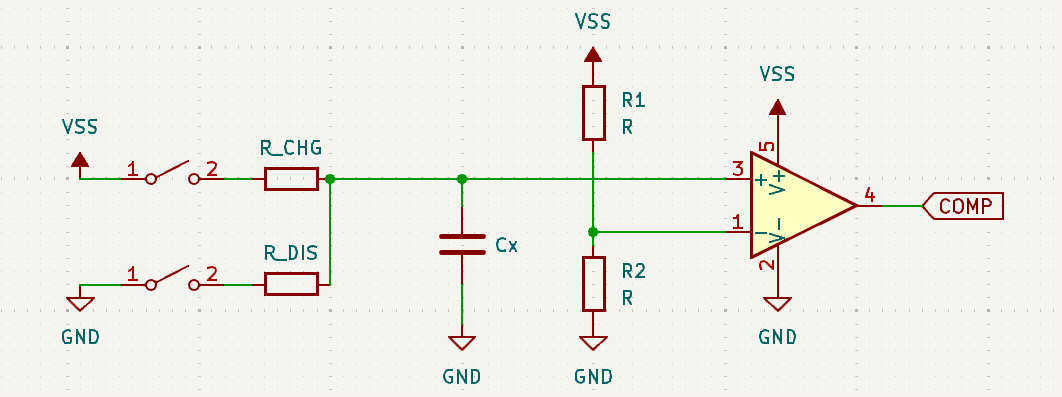
\includegraphics[width=\linewidth]{../thesis/fig/principle-cap-measure.png}
\end{figure}
\end{frame}


\begin{frame}{Soil Moisture Sensor}
\begin{columns}[T]
\begin{column}{.5\textwidth}
    \begin{figure}
        \centering
        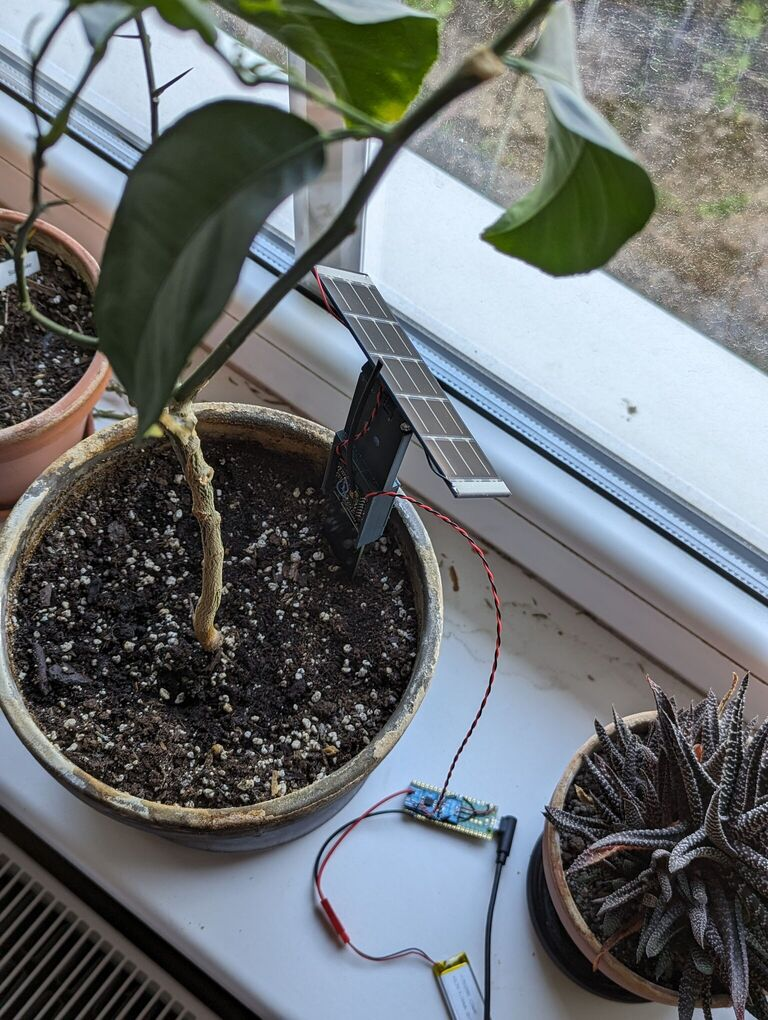
\includegraphics[width=\linewidth]{../thesis/img/sensor-deploy-up.jpg}
    \end{figure}
\end{column}
\hfil
\begin{column}{.5\textwidth}
    \begin{figure}
        \centering
        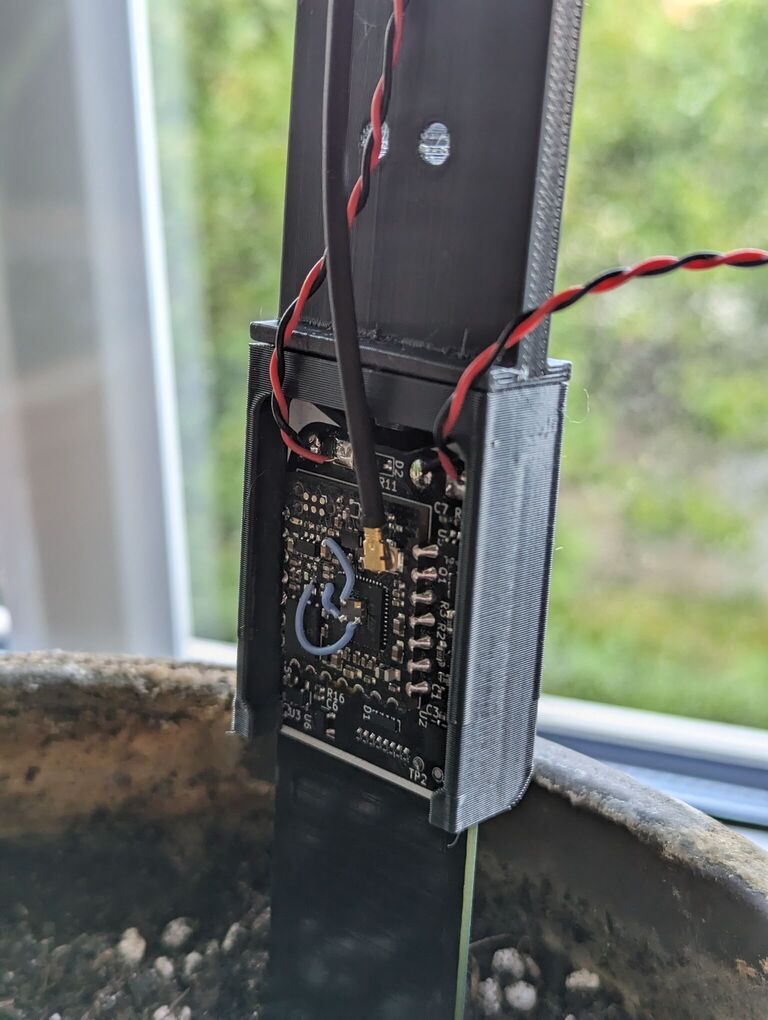
\includegraphics[width=\linewidth]{../thesis/img/sensor-deploy-close.jpg}
    \end{figure}
\end{column}
\end{columns}
\end{frame}





\end{document}
